\documentclass[handout]{beamer}
\usepackage{multicol}
\everymath{\displaystyle}
\mode<presentation>
{\usetheme{Warsaw}\setbeamercovered{dynamic}}
\usecolortheme{crane}
\usepackage{beamerfoils}
\pgfdeclareimage[height=1in]{university-logo}{ISULogo}
\logo{\pgfuseimage{university-logo}}
\setbeamertemplate{navigation symbols}{}
\title[\S3]{Section 3\\Odds}
\author{Dr Marcus Bishop}
\subject{Math 104}
\beamerdefaultoverlayspecification{<+->}
\theoremstyle{definition}
\newtheorem{remark}{Remark}
\newtheorem{impact}{Impact}
\newtheorem{notation}{Notation}
\usepackage{arev}
\begin{document}
\begin{frame}\titlepage\end{frame}
\LogoOff

\begin{frame}{Introduction}
\begin{itemize}
\item \alert{Odds} express same information as probability
\item In non-mathematical contexts
odds more common than probability
\end{itemize}
\begin{example}
\begin{itemize}
\item ``\alert{$1$ in $175,223,510$} the odds of winning Powerball''
\item ``Keselowski, who had a career-best Atlanta finish of third-place
during his 2012 Championship season, is one of the \alert{$6$-to-$1$} favorites''
\end{itemize}
\end{example}
\begin{remark}
\begin{itemize}
\item Odds consist of two numbers, separated by preposition \alert{in} or \alert{to}
\item Version with \alert{in} incorrect, according to textbook
\item Hyphens in second example make \alert{easier-to-read}
\end{itemize}
\end{remark}
\end{frame}

\begin{frame}{Odds against an event}
\begin{definition}
\begin{itemize}
\item $E$ an event
\item \alert{Odds against $E$} defined by
$\frac{P\left(\text{not $E$}\right)}{P\left(E\right)}$
\item Fraction must be written in \alert{lowest terms}
\item Then odds against $E$ often denoted by \alert{$X:Y$} or \alert{$X$-to-$Y$}
\item[]where $\frac{P\left(\text{not $E$}\right)}{P\left(E\right)}
=\frac{X}{Y}$ and $\frac{X}{Y}$ in lowest terms
\end{itemize}
\end{definition}
\end{frame}

\begin{frame}
\begin{example}
\begin{itemize}
\item Calculate odds against rolling $4$ on die
\item $P\left(\text{not $4$}\right)=5/6$
\item $P\left\{4\right\}=1/6$
\item Observe that $\frac{5/6}{1/6}=\frac{5}{1}$
\item So $5$-to-$1$ the odds against rolling $4$
\end{itemize}
\end{example}
\begin{remark}
\begin{itemize}
\item To divide fractions, multiply top fraction
by \alert{reciprocal} of bottom fraction
\item So
$\frac{5/6}{1/6}
\only<+->{=\frac{5}{6}\cdot\frac{6}{1}}\only<+->{=\frac{5}{1}}$
\item Can also skip middle step and ``cancel'' $1/6$ from
top and bottom
\end{itemize}
\end{remark}
\end{frame}

\begin{frame}{Chutes and Ladders revisited}
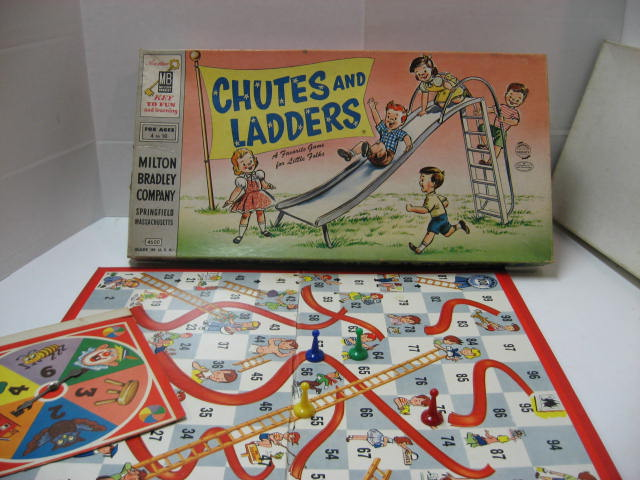
\includegraphics[scale=.22]{ChutesAndLadders}
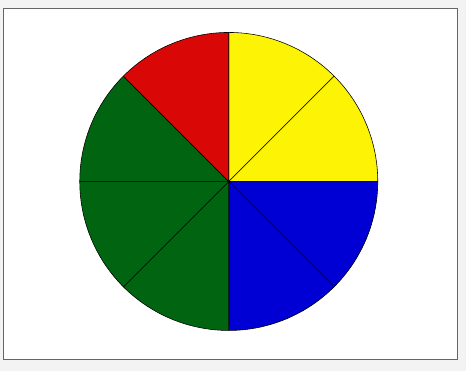
\includegraphics[scale=.30]{Spinner}
\begin{itemize}
\item Calculate odds against spinning green
\item Three of eight equally sized wedges green
\item So $P\left(\text{not green}\right)=5/8$
and $P\left(\text{green}\right)=3/8$
\item So $5:3$ the odds against green
\end{itemize}
\end{frame}

\begin{frame}{Odds in favor of $E$}
\begin{definition}
\begin{itemize}
\item \alert{Odds in favor of $E$} defined by
$\frac{P\left(E\right)}{P\left(\text{not $E$}\right)}$
\item Fraction should be reduced and written
in form \alert{$X:Y$} or \alert{$X$-to-$Y$}
where $X/Y$ in lowest terms
\end{itemize}
\end{definition}
\begin{example}
\begin{multicols}{2}
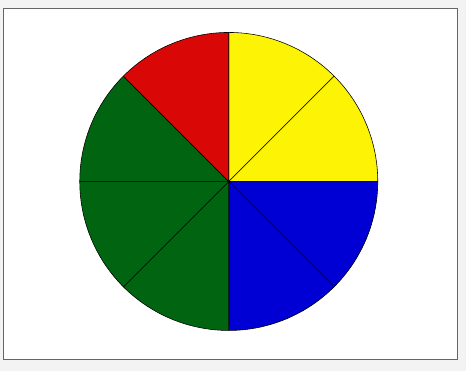
\includegraphics[scale=.30]{Spinner}
\begin{itemize}
\item $1/4$ the probability of spinning blue
\item $3/4$ the probability of \alert{not} spinning blue
\item $\frac{1/4}{3/4}=\frac{1}{3}$
\item So odds in favor of blue $1:3$
\end{itemize}
\end{multicols}
\end{example}
\end{frame}

\begin{frame}
\begin{itemize}
\item Odds against~$E$ more common than odds in favor of~$E$
\item Observe that odds in favor of~$E$ obtained
from odds against~$E$ by exchanging numbers
\begin{example} If $5:3$ the odds against spinning green,
then $3:5$ the odds in favor of green
\end{example}
\item Therefore very important to explicitly write
\alert{in favor} or \alert{against}
\item If neither mentioned, assume \alert{against}
\end{itemize}
\begin{example}
\begin{itemize}
\item ``Keselowski, who had a career-best Atlanta finish of third-place
during his 2012 Championship season, is one of the \alert{$6$-to-$1$} favorites''
\item Quotation clearly means $6:1$ the odds \alert{against} Keselowski
\end{itemize}
\end{example}
\end{frame}

\begin{frame}{Calculating probability from odds}
\begin{itemize}
\item If $X:Y$ the odds in favor of $E$
then $P\left(E\right)=\frac{X}{X+Y}$
\item If $X:Y$ the odds against $E$
then $P\left(E\right)=\frac{Y}{X+Y}$
\end{itemize}
\begin{example}
\begin{itemize}
\item $1:3$ the odds in favor of spinning blue
\item So $P\left(\text{blue}\right)=\frac{1}{1+3}=\frac{1}{4}$
\item Agrees with calculation above
\end{itemize}
\end{example}
\begin{example}
\begin{itemize}
\item $6:1$ the odds against Keselowski
\item So $\frac{1}{1+6}=\frac{1}{7}$ the probability
that Keselowski wins
\end{itemize}
\end{example}
\end{frame}

\begin{frame}{Interpretation of odds} 
\begin{itemize}
\item Suppose $5:3$ the odds against spinning green
\item Means that on average, for every five non-green outcomes
we expect $3$ green outcomes
\item Alternately, if spinner spun eight times, we expect
non-green $5$ times and green $3$ times on average
\item So odds justapose successes and failures by presenting
both numbers
\item In contrast, probability only highlights success
of experiment
\end{itemize}
\end{frame}

\begin{frame}
\begin{example}
\begin{itemize}
\item 1-in-175,223,510 the odds of winning
Iowa Lottery's Powerball
\item Interpretation: you win once for every
175,223,510 times you lose
\item Note that $100\cdot 365=36,500$ days in 100~years
\item So $\frac{175223510}{36000}\approx 4800$ people
playing Powerball every day for 100~years
might reasonably exect to win once
\end{itemize}
\end{example}
\begin{itemize}
\item This interpretation makes less sense in Nascar example
\item Suppose $6:1$ the odds against Keselowski
\item Then if race could be repeated seven times, he would
lose $6$ and win $1$ on average
\item Although race can't be repeated seven times,
still helpful to knows odds
\end{itemize}
\end{frame}

\begin{frame}{Diabetes (Exercise 54)}
\begin{itemize}
\item According to Centers for Disease Control
$8\%$ of Americans have diabetes
\item If American selected at random
calculate odds in favor that this person has diabetes
\item So $0.08$ the probability that randomly selected
American has diabetes
\item So $0.92$ the probability that randomly selected
American \alert{does not} has diabetes
\item $\frac{.08}{.92}
\only<+->{=\frac{8}{92}}
\only<+->{=\frac{2}{23}}$
\item So $2:23$ the odds in favor that randomly
selected American has diabetes
\end{itemize}
\end{frame}

\begin{frame}{Bookcase assembly (Exercise 55)}
\begin{multicols}{2}
\begin{itemize}
\item Suppose $7/8$ the probability that
all parts needed to assemble bookcase included in carton
\item Calculate odds against being able to assemble bookcase
\item $\frac{1/8}{7/8}=\frac{1}{7}$
\columnbreak
\item So $1:7$ the odds against being able to assemble bookcase
\end{itemize}
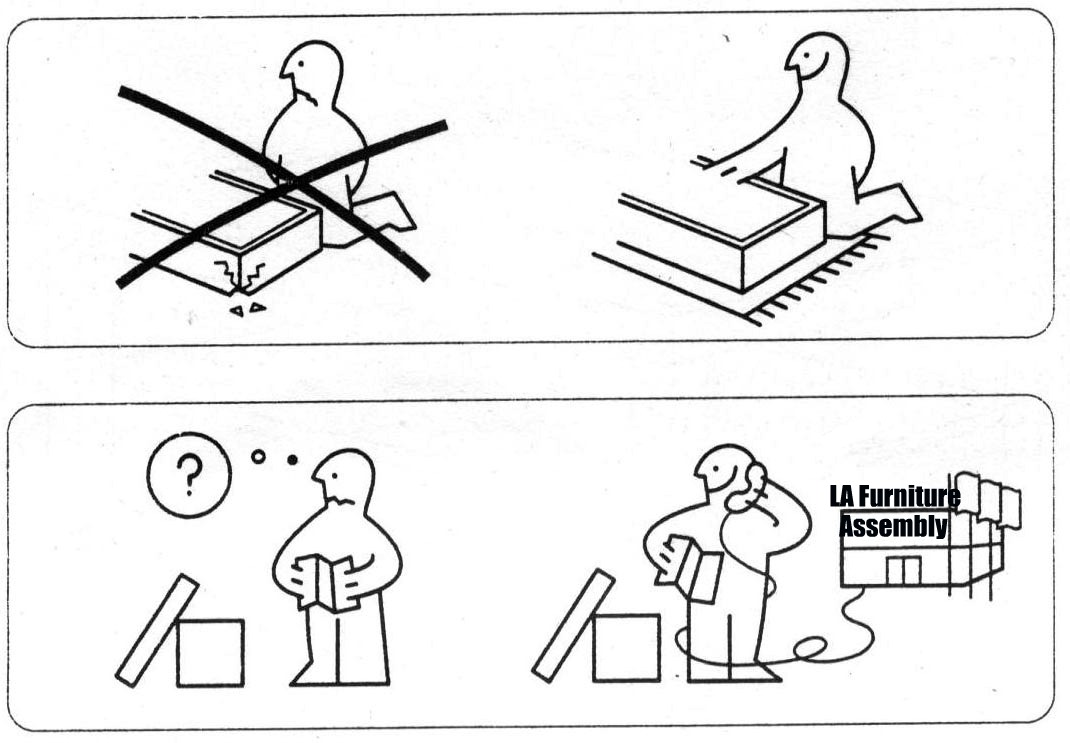
\includegraphics[scale=.15]{Ikea}
\end{multicols}
\end{frame}


\end{document}
